%%%%%%%%%%%%%%%%%%%%%%%%%%%%%%%%%%%%%%%%%%%%%%%%%%%%%%%%%%%%%%%%%%%%%%%%%%%%%%%%
%2345678901234567890123456789012345678901234567890123456789012345678901234567890
%        1         2         3         4         5         6         7         8

\documentclass[letterpaper, 10 pt, conference]{ieeeconf}  % Comment this line out if you need a4paper

%\documentclass[a4paper, 10pt, conference]{ieeeconf}      % Use this line for a4 paper

\IEEEoverridecommandlockouts                              % This command is only needed if 
                                                          % you want to use the \thanks command

\overrideIEEEmargins                                      % Needed to meet printer requirements.

% See the \addtolength command later in the file to balance the column lengths
% on the last page of the document

% The following packages can be found on http:\\www.ctan.org
\usepackage{graphics} % for pdf, bitmapped graphics files
\usepackage{epsfig} % for postscript graphics files
\usepackage{mathptmx} % assumes new font selection scheme installed
\usepackage{times} % assumes new font selection scheme installed
\usepackage{amsmath} % assumes amsmath package installed
\usepackage{amssymb}  % assumes amsmath package installed
	
\title{\LARGE \bf
Structure of the set of feasible neural commands for complex motor tasks*
}

\author{TODOFCO(choose authors and order)$^{1}$ and Bernard D. Researcher$^{2}$% <-this % stops a space
\thanks{*This work was supported by TODOFCO(add funding)}% <-this % stops a space
\thanks{$^{1}$Brian Cohn is with the departments of Biomedical Engineering and Computer Science at the University of Southern California Viterbi School of Engineering, Los Angeles, CA 90089, USA
        {\tt\small brianaco@usc.edu}}%
\thanks{$^{2}$Francisco is from TODOFCO
        {\tt\small valero@usc.edu}}%
}


\begin{document}



\maketitle
\thispagestyle{empty}
\pagestyle{empty}


%%%%%%%%%%%%%%%%%%%%%%%%%%%%%%%%%%%%%%%%%%%%%%%%%%%%%%%%%%%%%%%%%%%%%%%%%%%%%%%%
\begin{abstract}
The brain must select its control strategies among an infinite set of possibilties, thereby solving an optimization problem. 
While this set is infinite and lies in high dimensions, it is bounded by kinematic, neuromuscular, and anatomical constraints, within which the brain must select optimal solutions. 
We use data from a human index finger with 7 muscles, 4DOF, and 4 output dimensions. For a given force vector at the endpoint, the feasible activation space is a 3D convex polytope, embedded in the 7D unit cube.
It is known that explicitly computing the volume of this polytope can become too computationally complex in many instances. 
We generated random points in the feasible activation space using the Hit-and-Run method, which converged to the uniform distribution. 
After generating enough points, we computed the distribution of activation across each muscle, shedding light onto the structure of these solution spaces- rather than simply exploring their maximal and nimimal values. 
Although this paper presents a 7 dimensional case of the index finger, our methods extend to systems with up to at least 40 muscles. We challenge the community to map the shapes distributions of each variable in the solution space, thereby providing important contextual information into optimization of motor cortical function in future research.
\end{abstract}
%%%%%%%%%%%%%%%%%%%%%%%%%%%%%%%%%%%%%%%%%%%%%%%%%%%%%%%%%%%%%%%%%%%%%%%%%%%%%%%%
\begin{introduction}
\section{INTRODUCTION}

Muscle redundancy is the term used to describe the underdetermined nature of neural control of musculature.
The classical notion of muscle redundancy  proposes that, faced with an infinite number of possible muscle activation patterns for a given task, the nervous system uses optimization to select a given specific solution.
Here, each of the $N$ muscles represents a dimension of control, and a muscle activation pattern is a point in $\mathbb{R}^N$ \cite{Valero-Cuevas1998Large}.
Thus researchers often seek to infer the optimization approach and the costs functions the nervous system likely utilizes to find the points in activation space to produce natural behavior\cite{Chao1978Graphical,Prilutsky2000Muscle,scott2004optimal,todorov2002optimal,crowninshield1981physiologically,higginson2005simulated}. 


Implicit in these optimization procedures is the notion that there exists a well structured set of feasible solutions. Thus several of us have focused on describing and understanding those high-dimensional subspaces  embedded in $\mathbb{R}^N$ \cite{kutch2011muscle,kutch2012challenges,sohn2013cat_bounding_box,Valero-Cuevas1998Large,Valero-Cuevas2015high-dimensional}.

For the case of muscle redundancy for submaximal and static force production with a limb,  the problem is phrased as one of computational geometry: find the convex polytope of feasible muscle activations given the mechanics of the limb and the constrains of the task \cite{avis1992Pivoting,Valero-Cuevas1998Large,Valero-Cuevas2009mathematical,Valero-Cuevas2015high-dimensional}.  To date, the structure of this high-dimensional polytope is to characterize its bounding box \cite{kutch2011muscle,sohn2013cat_bounding_box,Valero-Cuevas2015high-dimensional}.  But the bounding box of a convex polytope will always overestimate its volume, and lose the details of its shape.  Empirical dimensionality-reduction methods have also been used to calculate a basis for the subspace \cite{Clewley2008Estimating,davella2005shared,krishnamoorthy2003muscle}. Those basis vectors  provide a description of the dimension, orientation, and aspect ratio of the polytope, but not of its vertices, faces, or structure.

Here we present a novel approach based on combinatorial redundancy detection \cite{fukuda2014combinatorial} to describe the internal structure of these high-dimensional polytopes of feasible muscle activation patterns.
\begin{itemize}

\item first claim
\item second claim
\item third claim

\end{itemize}

\end{introduction}
\section{Materials and Methods}


\Section{RESULTS}

Figure \ref{fig:raw_histograms} shows the distributions of activations resulting from $1,000,000$ iterations of the Hit-And-Run algorithm. To our knowledge, this is 

\begin{figure}[htbp]
\centering
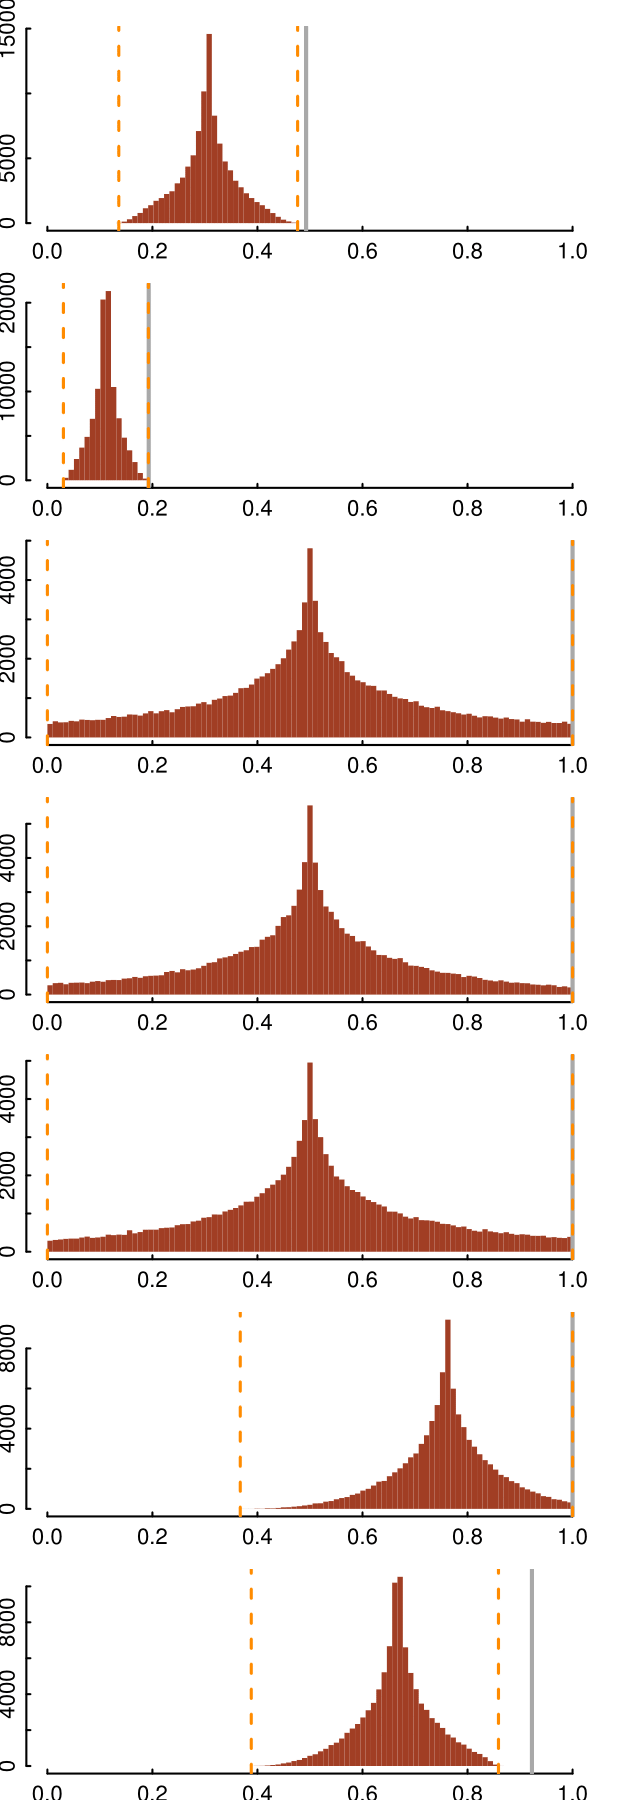
\includegraphics[width=7.5cm\textwidth]{sections/figs/raw_histograms.png}
\caption{My Nice Figure.}
\label{fig:raw_histograms}
\end{figure}

\section{DISCUSSION}

Our results clearly show that\\
-The Hit-and-Run algorithm can explore the feasible activation space for a realistic 7-muscle finger in a way that is computationally tractable.\\
-For some muscles, we find that the bounding box exceptionally misconstrues the internal structure of the feasible activation set.\\
-The Hit-and-Run algorithm is cost-agnostic in the sense that no cost function is needed to predict the distribution of muscle activation patterns. Therefore, we can provide spatial context to where 'optimal' solutions lie within the solution space; this approach can be used to explore the consequences of different cost functions.\\
-The distribution of muscle activations often show and strong modes that will critically affect the learning of motor tasks.


If the feasible activation space is skewed or condensed, we can learn about the statistical tendencies of the musculoskeletal system, and better define the plane upon which optimization occurs. This application of Hit-and-Run provides a tool to generate testable hypotheses of how coordination habits may come about, how they are learned, and how difficult or easy it is to break out of them. 




\section{PROCEDURE FOR PAPER SUBMISSION}

\subsection{Selecting a Template (Heading 2)}

First, confirm that you have the correct template for your paper size. This template has been tailored for output on the US-letter paper size. 
It may be used for A4 paper size if the paper size setting is suitably modified.

\subsection{Maintaining the Integrity of the Specifications}

The template is used to format your paper and style the text. All margins, column widths, line spaces, and text fonts are prescribed; please do not alter them. You may note peculiarities. For example, the head margin in this template measures proportionately more than is customary. This measurement and others are deliberate, using specifications that anticipate your paper as one part of the entire proceedings, and not as an independent document. Please do not revise any of the current designations

\section{MATH}

Before you begin to format your paper, first write and save the content as a separate text file. Keep your text and graphic files separate until after the text has been formatted and styled. Do not use hard tabs, and limit use of hard returns to only one return at the end of a paragraph. Do not add any kind of pagination anywhere in the paper. Do not number text heads-the template will do that for you.

$$
\alpha + \beta = \chi \eqno{(1)}
$$


\subsection{Figures and Tables}

Positioning Figures and Tables: Place figures and tables at the top and bottom of columns. Avoid placing them in the middle of columns. Large figures and tables may span across both columns. Figure captions should be below the figures; table heads should appear above the tables. Insert figures and tables after they are cited in the text. Use the abbreviation �Fig. 1�, even at the beginning of a sentence.

\begin{table}[h]
\caption{An Example of a Table}
\label{table_example}
\begin{center}
\begin{tabular}{|c||c|}
\hline
One & Two\\
\hline
Three & Four\\
\hline
\end{tabular}
\end{center}
\end{table}


   \begin{figure}[thpb]
      \centering
      \framebox{\parbox{3in}{We suggest that you use a text box to insert a graphic (which is ideally a 300 dpi TIFF or EPS file, with all fonts embedded) because, in an document, this method is somewhat more stable than directly inserting a picture.
}}
      %\includegraphics[scale=1.0]{figurefile}
      \caption{Inductance of oscillation winding on amorphous
       magnetic core versus DC bias magnetic field}
      \label{figurelabel}
   \end{figure}
  

\addtolength{\textheight}{-12cm}   % This command serves to balance the column lengths
                                  % on the last page of the document manually. It shortens
                                  % the textheight of the last page by a suitable amount.
                                  % This command does not take effect until the next page
                                  % so it should come on the page before the last. Make
                                  % sure that you do not shorten the textheight too much.

%%%%%%%%%%%%%%%%%%%%%%%%%%%%%%%%%%%%%%%%%%%%%%%%%%%%%%%%%%%%%%%%%%%%%%%%%%%%%%%%



%%%%%%%%%%%%%%%%%%%%%%%%%%%%%%%%%%%%%%%%%%%%%%%%%%%%%%%%%%%%%%%%%%%%%%%%%%%%%%%%



%%%%%%%%%%%%%%%%%%%%%%%%%%%%%%%%%%%%%%%%%%%%%%%%%%%%%%%%%%%%%%%%%%%%%%%%%%%%%%%%
\section*{APPENDIX}

NA for now

\section*{ACKNOWLEDGMENT}

@FCO(Insert ETH funding ack.)


%%%%%%%%%%%%%%%%%%%%%%%%%%%%%%%%%%%%%%%%%%%%%%%%%%%%%%%%%%%%%%%%%%%%%%%%%%%%%%%%

References are important to the reader; therefore, each citation must be complete and correct. If at all possible, references should be commonly available publications.

\bibliographystyle{plain}
\bibliography{ieee}


\end{document}
